% Pedal Trinity - Guida illustrata
% Copyright (C) 2026 FabioNET - GNU GPL v3
% Compilazione: xelatex PedalTrinity_Guida.tex (due passaggi)
\documentclass[11pt,a4paper]{article}
\usepackage{fontspec}
\setmainfont{Lato}[UprightFont=*-Regular,BoldFont=*-Bold,ItalicFont=*-Italic,BoldItalicFont=*-BoldItalic,
  Path=/usr/share/fonts/truetype/lato/, Extension=.ttf]
\newfontfamily\heavy{Lato-Black}[Path=/usr/share/fonts/truetype/lato/, Extension=.ttf,
  ItalicFont=Lato-BlackItalic]
\setmonofont{DejaVuSansMono}[Path=/usr/share/fonts/truetype/dejavu/, Extension=.ttf, Scale=0.88,
  BoldFont=DejaVuSansMono-Bold]
\usepackage[a4paper,margin=2.1cm,top=2.4cm,bottom=2.4cm]{geometry}
\usepackage{graphicx,xcolor,tikz,booktabs,tabularx,enumitem,fancyhdr,titlesec,ragged2e}
\usepackage[most]{tcolorbox}
\usepackage[hidelinks,pdftitle={Pedal Trinity - Guida},pdfauthor={FabioNET}]{hyperref}
\usetikzlibrary{arrows.meta,positioning,shadows}

\definecolor{emerald}{HTML}{268040}
\definecolor{charcoal}{HTML}{1E1E21}
\definecolor{orange}{HTML}{F0781E}
\definecolor{gold}{HTML}{C9A44E}
\definecolor{steel}{HTML}{8C9098}
\definecolor{eqblue}{HTML}{143C96}
\definecolor{paper}{HTML}{F6F5F1}

\RaggedRight
\hyphenpenalty=10000
\setlength{\parskip}{0.55em}
\setlength{\parindent}{0pt}
\setlist{itemsep=0.2em,topsep=0.3em}

\titleformat{\section}{\heavy\LARGE\color{charcoal}}{\color{emerald}\thesection}{0.6em}{}[\vspace{-0.3em}{\color{gold}\rule{\linewidth}{1.2pt}}]
\titleformat{\subsection}{\bfseries\Large\color{charcoal}}{\thesubsection}{0.5em}{}
\titlespacing*{\section}{0pt}{1.2em}{0.8em}

\pagestyle{fancy}
\fancyhf{}
\fancyhead[L]{\small\color{steel}\textbf{PEDAL TRINITY} \,·\, Guida all'uso}
\fancyhead[R]{\small\color{steel}v1.0.0 beta}
\fancyfoot[L]{\small\color{steel}© 2026 FabioNET \,·\, GNU GPL v3}
\fancyfoot[R]{\small\color{steel}\thepage}
\renewcommand{\headrulewidth}{0.4pt}
\renewcommand{\headrule}{\color{steel!50}\hrule width\headwidth height\headrulewidth}

\newtcolorbox{nota}[1][Suggerimento]{enhanced,colback=emerald!6,colframe=emerald!70!black,
  fonttitle=\bfseries,title=#1,arc=2mm,boxrule=0.7pt,left=3mm,right=3mm}
\newtcolorbox{avviso}[1][Attenzione]{enhanced,colback=orange!8,colframe=orange!80!black,
  fonttitle=\bfseries,title=#1,arc=2mm,boxrule=0.7pt,left=3mm,right=3mm}
\newcommand{\num}[1]{\tikz[baseline=(n.base)]\node[circle,fill=gold,text=black,inner sep=1.2pt,
  minimum size=1.25em,font=\footnotesize\bfseries](n){#1};}
\newcommand{\ctl}[1]{\textbf{\textsf{#1}}}

\renewcommand{\contentsname}{Indice}
\begin{document}

% ------------------------------------------------------------------ copertina
\begin{titlepage}
\newgeometry{margin=0cm}
\pagecolor{charcoal}\color{white}
\begin{tikzpicture}[remember picture,overlay]
  \node[anchor=north,inner sep=0] at ([yshift=-3.2cm]current page.north)
      {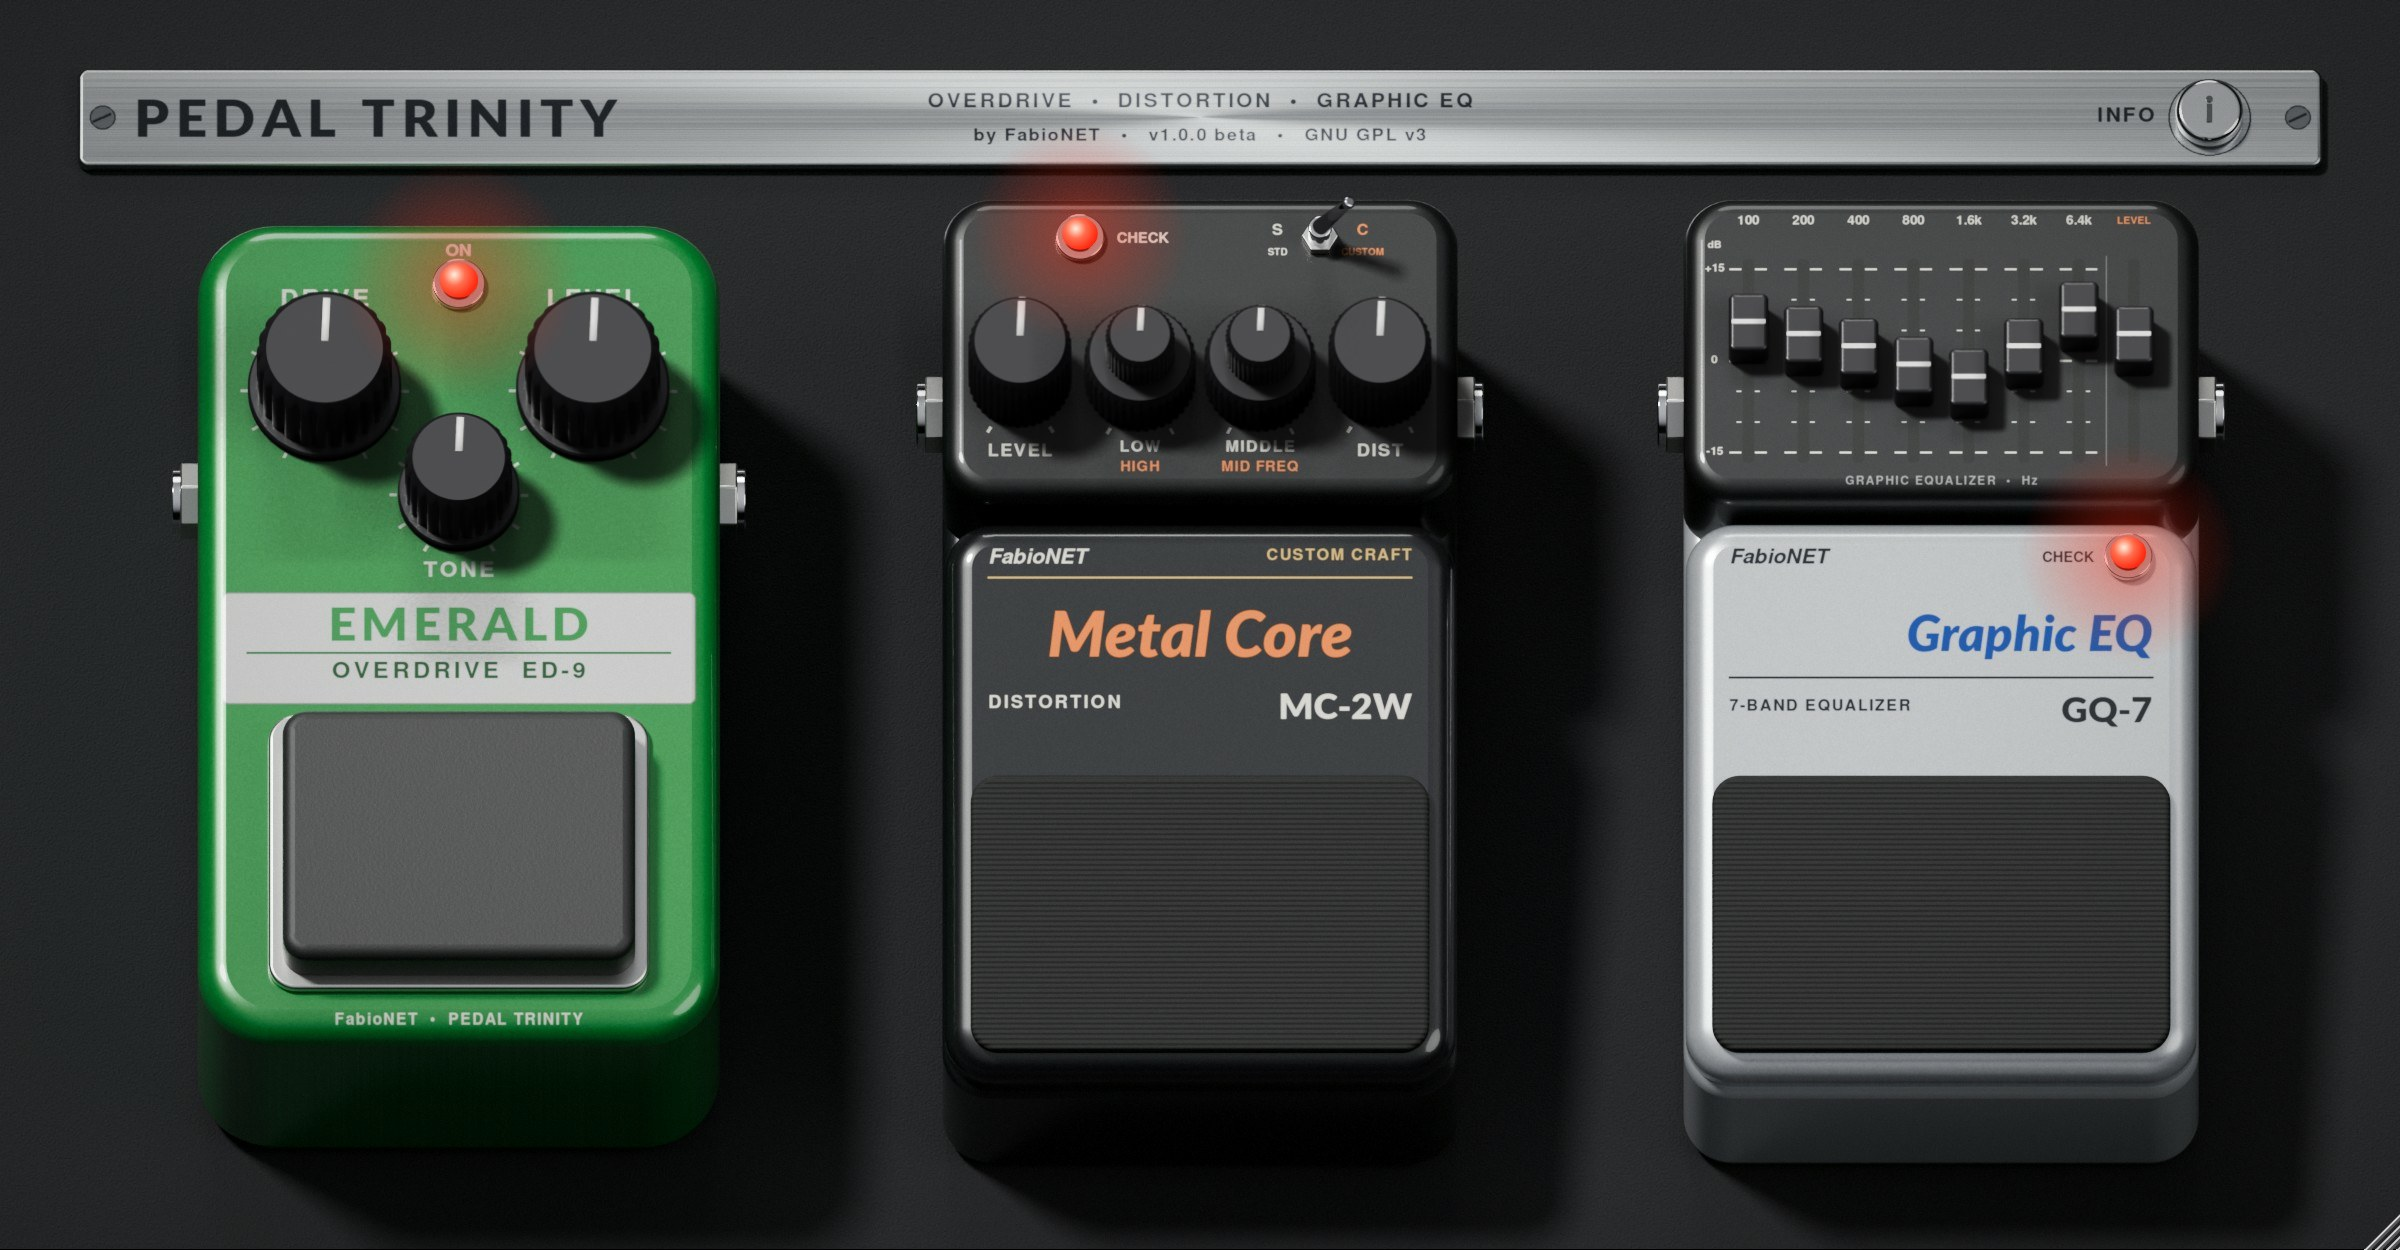
\includegraphics[width=\paperwidth]{../images/cover.jpg}};
  \node[anchor=north west,text width=17cm,align=left,text=white] at ([xshift=2cm,yshift=-15.2cm]current page.north west)
      {{\heavy\fontsize{54}{58}\selectfont PEDAL TRINITY}\\[0.6em]
       {\Large\color{gold}Overdrive \,·\, Distorsore \,·\, Equalizzatore grafico}\\[2.2em]
       {\LARGE\bfseries Guida illustrata all'uso}\\[0.4em]
       {\large Versione 1.0.0 beta}};
  \node[anchor=south west,text width=17cm,align=left,text=white] at ([xshift=2cm,yshift=2.2cm]current page.south west)
      {\large by \textbf{FabioNET}\\[0.3em]
       \color{white!70}Plugin VST3 \,·\, LV2 \,·\, Standalone \quad per Linux e Windows (ASIO)\\
       Software libero rilasciato con licenza GNU General Public License v3};
\end{tikzpicture}
\end{titlepage}
\restoregeometry
\nopagecolor\color{black}

\tableofcontents
\vspace{1em}
\begin{nota}[In breve]
Pedal Trinity riunisce tre pedali per chitarra in un unico plugin con un'interfaccia fotorealistica:
l'overdrive \textbf{Emerald Drive ED-9}, il distorsore \textbf{Metal Core MC-2W} e l'equalizzatore
grafico \textbf{Graphic EQ GQ-7}. Si usa come plugin VST3 o LV2 nella tua DAW oppure come applicazione
indipendente (Standalone) collegando la chitarra alla scheda audio.
\end{nota}

% ------------------------------------------------------------------
\section{Introduzione}
Pedal Trinity riproduce una piccola pedaliera: tre pedali collegati in serie, ognuno con il proprio
interruttore a pedale e il proprio LED. I comandi sono quelli dei pedali reali: pomelli da ruotare,
cursori da far scorrere e interruttori da premere.

\begin{center}
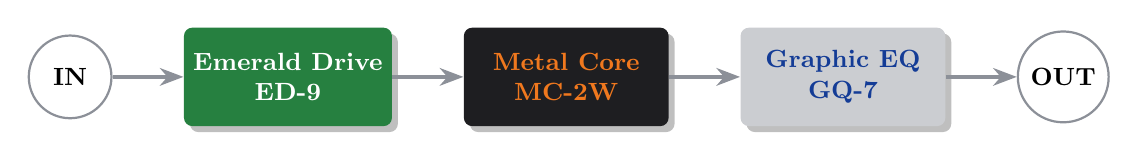
\begin{tikzpicture}[node distance=0.9cm,
  box/.style={draw=none,rounded corners=3pt,minimum width=2.6cm,minimum height=1.25cm,align=center,
              font=\bfseries\small,drop shadow},
  io/.style={circle,draw=steel,thick,minimum size=1.05cm,font=\bfseries\small},
  arr/.style={-{Stealth[length=3mm]},very thick,color=steel}]
  \node[io] (in) {IN};
  \node[box,fill=emerald,text=white,right=of in] (ts) {Emerald Drive\\ED-9};
  \node[box,fill=charcoal,text=orange,right=of ts] (mt) {Metal Core\\MC-2W};
  \node[box,fill=steel!45,text=eqblue,right=of mt] (eq) {Graphic EQ\\GQ-7};
  \node[io,right=of eq] (out) {OUT};
  \draw[arr] (in) -- (ts); \draw[arr] (ts) -- (mt); \draw[arr] (mt) -- (eq); \draw[arr] (eq) -- (out);
\end{tikzpicture}
\end{center}

\begin{tabularx}{\linewidth}{@{}l X X@{}}
\toprule
\textbf{Pedale} & \textbf{Ispirato a} & \textbf{Carattere} \\ \midrule
Emerald Drive ED-9 & Ibanez Tube Screamer (TS808/TS9) & overdrive caldo con medie in evidenza, bassi puliti \\
Metal Core MC-2W & BOSS MT-2W Metal Zone Waza Craft & distorsione ad alto guadagno con EQ attivo a 3 bande \\
Graphic EQ GQ-7 & BOSS GE-7 & equalizzatore grafico a 7 bande $\pm$15\,dB \\ \bottomrule
\end{tabularx}

Alla prima apertura sono accesi l'overdrive e l'equalizzatore (piatto); il distorsore è spento.

% ------------------------------------------------------------------
\section{Installazione}
\subsection{Linux (pacchetto .deb)}
Il pacchetto funziona su Ubuntu 22.04 o successivi, Debian 12, Linux Mint 21 e distribuzioni derivate
(64 bit). Da terminale, nella cartella in cui hai scaricato il file:
\begin{tcolorbox}[colback=charcoal,colupper=white,boxrule=0pt,arc=2mm]
\texttt{sudo apt install ./pedal-trinity\_1.0.0\textasciitilde beta-1\_amd64.deb}
\end{tcolorbox}
Vengono installati:
\begin{itemize}
  \item il plugin VST3 in \texttt{/usr/lib/vst3/Pedal Trinity.vst3};
  \item il plugin LV2 in \texttt{/usr/lib/lv2/Pedal Trinity.lv2};
  \item l'applicazione \texttt{pedal-trinity}, che trovi nel menu \emph{Audio/Multimedia};
  \item questa guida in \texttt{/usr/share/doc/pedal-trinity/}.
\end{itemize}
Per disinstallare: \texttt{sudo apt remove pedal-trinity}.

\subsection{Windows 10/11 (installer)}
Avvia \texttt{PedalTrinity-1.0.0-beta-Windows-x64-Setup.exe} e segui la procedura (in italiano).
Puoi scegliere quali componenti installare:
\begin{itemize}
  \item \textbf{Standalone} in \texttt{C:\textbackslash Program Files\textbackslash Pedal Trinity}, con supporto ai driver \textbf{ASIO};
  \item \textbf{VST3} in \texttt{C:\textbackslash Program Files\textbackslash Common Files\textbackslash VST3};
  \item \textbf{LV2} in \texttt{C:\textbackslash Program Files\textbackslash Common Files\textbackslash LV2}.
\end{itemize}
Nel menu Start trovi l'app, questa guida e il testo della licenza.

\subsection{Nella DAW}
Dopo l'installazione, fai ripetere alla DAW la scansione dei plugin (Reaper, Ardour, Bitwig, Cubase,
Studio One, Carla, LMMS\dots). Pedal Trinity compare fra gli effetti di distorsione del produttore
\textbf{FabioNET}. Inseriscilo su una traccia mono o stereo con la chitarra registrata in diretta (DI).

% ------------------------------------------------------------------
\clearpage
\section{L'interfaccia}
\begin{center}
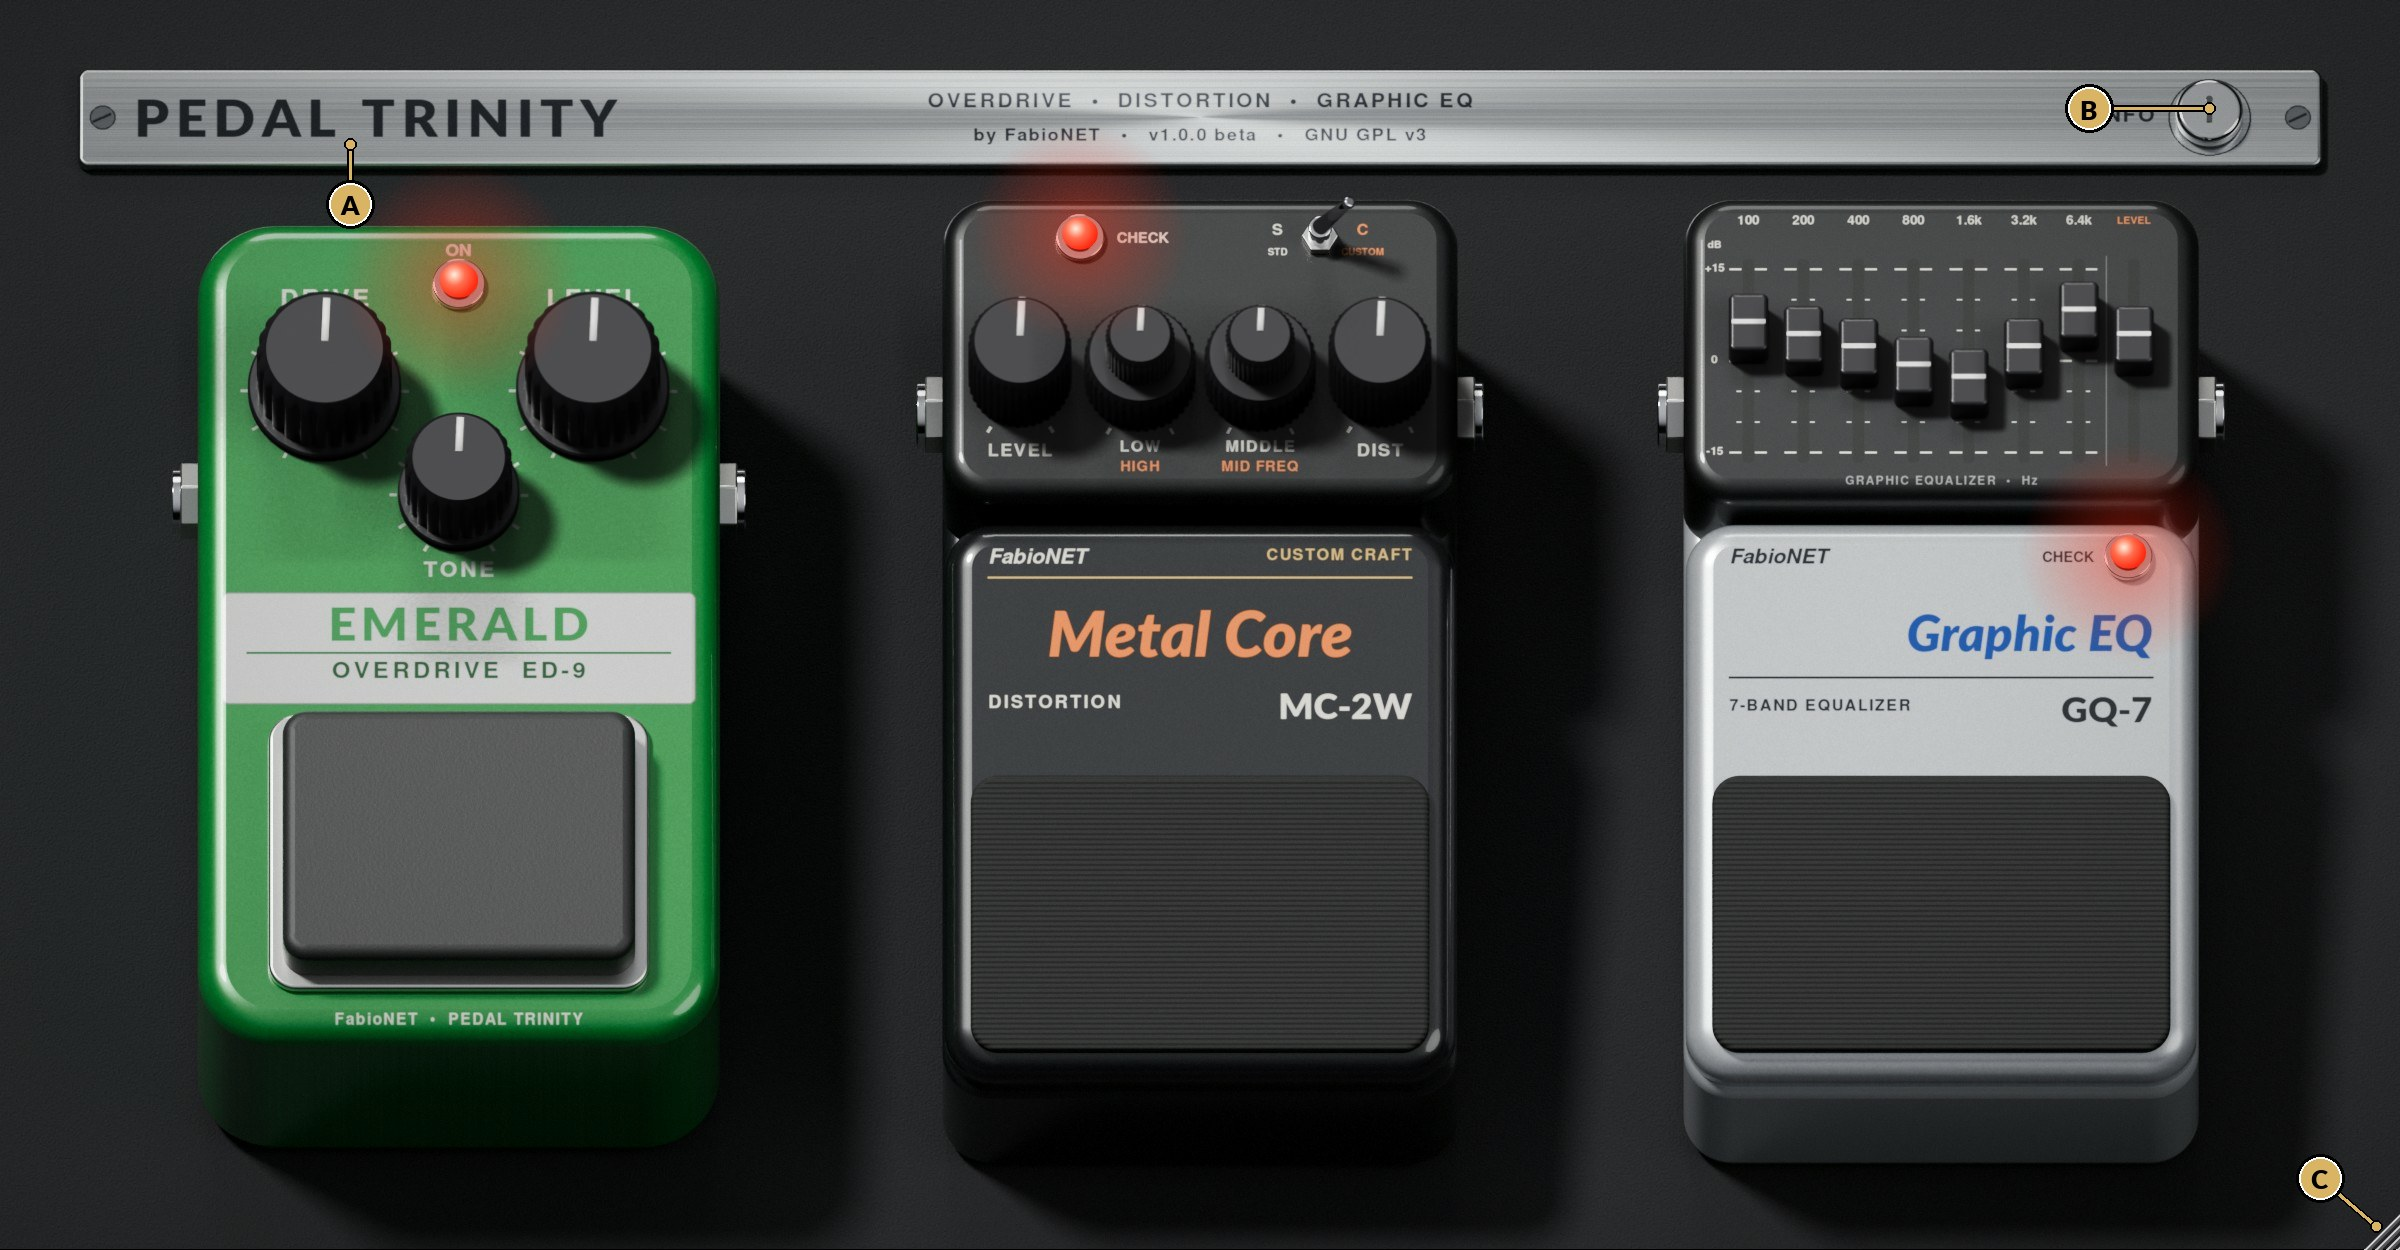
\includegraphics[width=\linewidth]{../images/guide_overview.jpg}
\end{center}
\begin{itemize}
  \item \num{A} \textbf{Targhetta}: nome del prodotto, versione e autore.
  \item \num{B} \textbf{Tasto INFO}: apre la finestra con licenza, crediti e il pulsante per aprire questa guida.
  \item \num{C} \textbf{Angolo di ridimensionamento}: trascinalo per ingrandire o ridurre la finestra
        (dal 50\% al 200\%); le proporzioni restano fisse.
\end{itemize}

\begin{nota}[Come si usano i comandi]
\begin{itemize}[leftmargin=1.2em]
  \item \textbf{Pomelli}: clicca e trascina in \emph{verticale} (verso l'alto aumenta) o in orizzontale; puoi usare anche la rotella del mouse.
  \item \textbf{Cursori} dell'equalizzatore: trascina in su o in giù.
  \item \textbf{Doppio clic} su un pomello o un cursore: torna al valore di fabbrica.
  \item Durante la regolazione appare un \textbf{fumetto} con il valore esatto (es.\ \texttt{DRIVE 6.3}, \texttt{800 Hz +4.5 dB}).
  \item \textbf{Footswitch}: clicca sul pedale per accenderlo o spegnerlo; il LED rosso indica che è attivo.
\end{itemize}
\end{nota}

% ------------------------------------------------------------------
\clearpage
\section{Emerald Drive ED-9 (overdrive)}
\begin{minipage}[t]{0.44\linewidth}\vspace{0pt}
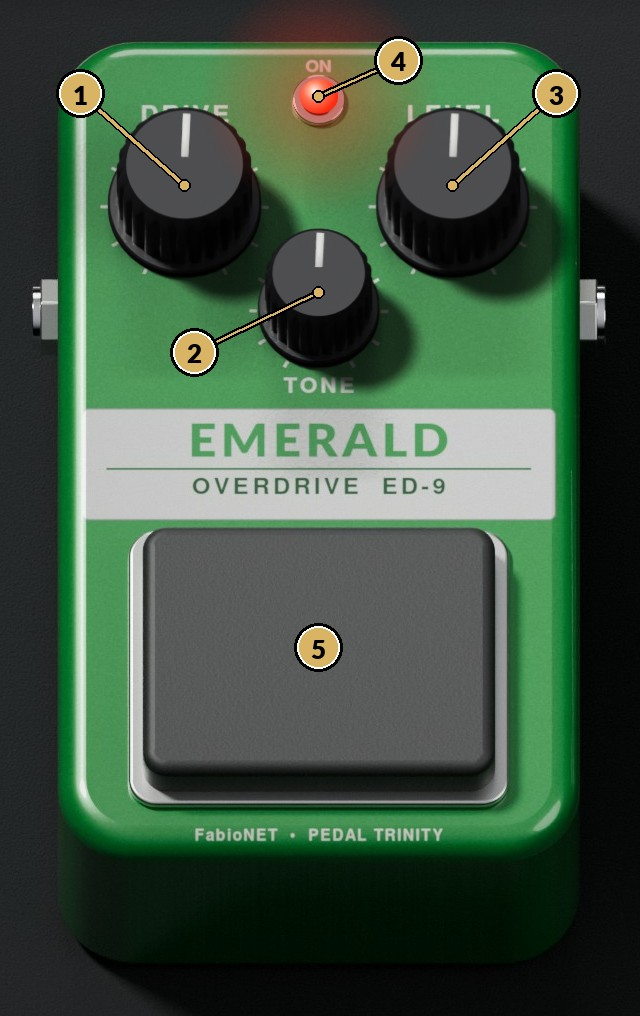
\includegraphics[width=\linewidth]{../images/guide_ed9.jpg}
\end{minipage}\hfill
\begin{minipage}[t]{0.52\linewidth}\vspace{0pt}
Il classico overdrive verde: l'amplificazione agisce soprattutto sulle frequenze medie mentre i bassi
passano puliti. Il risultato è un suono caldo e definito, perfetto per spingere un amplificatore già
saturo o il distorsore che segue.

\begin{tabularx}{\linewidth}{@{}l l X@{}}
\toprule
& \textbf{Comando} & \textbf{Funzione} \\ \midrule
\num{1} & \ctl{DRIVE} & quantità di saturazione (0–10) \\
\num{2} & \ctl{TONE} & timbro: da scuro (0) a brillante (10) \\
\num{3} & \ctl{LEVEL} & volume d'uscita; a 5 circa il livello d'ingresso \\
\num{4} & \ctl{LED ON} & acceso quando il pedale è attivo \\
\num{5} & \ctl{Footswitch} & accende/spegne il pedale \\ \bottomrule
\end{tabularx}
\end{minipage}

\begin{nota}[Il trucco del «boost»]
Imposta \ctl{DRIVE} a 0–2, \ctl{TONE} a 5–6 e \ctl{LEVEL} a 7–9, poi accendi anche il Metal Core:
l'ED-9 stringe i bassi e rende la distorsione più precisa, come fanno molti chitarristi metal.
\end{nota}

% ------------------------------------------------------------------
\clearpage
\section{Metal Core MC-2W (distorsore)}
\begin{minipage}[t]{0.44\linewidth}\vspace{0pt}
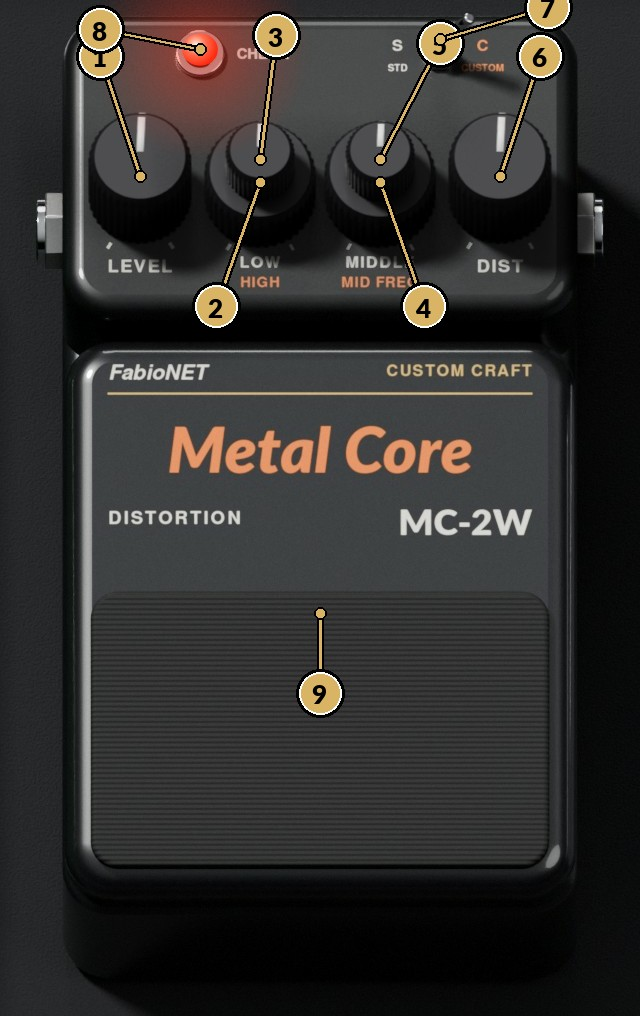
\includegraphics[width=\linewidth]{../images/guide_mc2.jpg}
\end{minipage}\hfill
\begin{minipage}[t]{0.52\linewidth}\vspace{0pt}
Distorsione ad alto guadagno con due stadi di saturazione ed equalizzatore attivo a tre bande con medie
parametriche. I due pomelli centrali sono \textbf{concentrici}: l'anello esterno e il pomello interno
regolano due parametri diversi.

\begin{tabularx}{\linewidth}{@{}l l X@{}}
\toprule
& \textbf{Comando} & \textbf{Funzione} \\ \midrule
\num{1} & \ctl{LEVEL} & volume d'uscita \\
\num{2} & \ctl{LOW} (anello) & bassi $\pm$15\,dB (100\,Hz) \\
\num{3} & \ctl{HIGH} (interno) & alti $\pm$15\,dB (6\,kHz) \\
\num{4} & \ctl{MIDDLE} (anello) & medie $\pm$15\,dB \\
\num{5} & \ctl{MID FREQ} (int.) & frequenza delle medie 200\,Hz–5\,kHz \\
\num{6} & \ctl{DIST} & quantità di distorsione \\
\num{7} & \ctl{S / C} & modo Standard o Custom \\
\num{8} & \ctl{CHECK} & LED di pedale attivo \\
\num{9} & \ctl{Pedale} & accende/spegne \\ \bottomrule
\end{tabularx}
\end{minipage}

\subsection*{Modo S e modo C}
Clicca sulla \textbf{levetta} \num{7} per cambiare modo.
\begin{itemize}
  \item \textbf{S (Standard)}: timbro aggressivo e tagliente, con il tipico picco sulle medie.
  \item \textbf{C (Custom)}: più guadagno, bassi più compatti e acuti più morbidi, con una saturazione più rotonda: ideale per ritmiche moderne e assoli.
\end{itemize}
\begin{nota}[Per ritmiche «scooped»]
\ctl{MIDDLE} a –8\,dB con \ctl{MID FREQ} verso 600–800\,Hz, \ctl{LOW} e \ctl{HIGH} a +3/+5\,dB.
Per gli assoli fai l'opposto: \ctl{MIDDLE} a +6\,dB intorno a 1\,kHz.
\end{nota}

% ------------------------------------------------------------------
\clearpage
\section{Graphic EQ GQ-7 (equalizzatore)}
\begin{minipage}[t]{0.44\linewidth}\vspace{0pt}
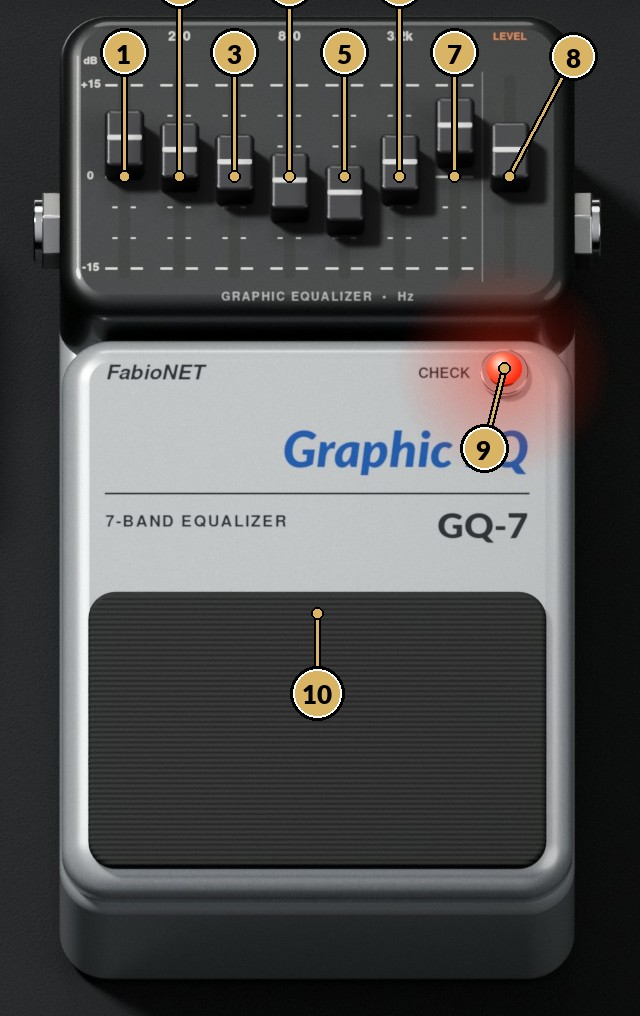
\includegraphics[width=\linewidth]{../images/guide_gq7.jpg}
\end{minipage}\hfill
\begin{minipage}[t]{0.52\linewidth}\vspace{0pt}
Equalizzatore grafico a 7 bande: ogni cursore alza o abbassa di al massimo 15\,dB la propria banda di
frequenze. Il cursore \ctl{LEVEL} regola il volume generale.

\begin{tabularx}{\linewidth}{@{}l l X@{}}
\toprule
& \textbf{Cursore} & \textbf{Zona} \\ \midrule
\num{1} & 100\,Hz & corpo, «pugno» sui bassi \\
\num{2} & 200\,Hz & calore, rimbombo \\
\num{3} & 400\,Hz & pienezza, «scatola» \\
\num{4} & 800\,Hz & medie, presenza nel mix \\
\num{5} & 1.6\,kHz & attacco, definizione \\
\num{6} & 3.2\,kHz & mordente, articolazione \\
\num{7} & 6.4\,kHz & brillantezza, fruscio \\
\num{8} & LEVEL & volume $\pm$15\,dB \\
\num{9} & CHECK & LED di pedale attivo \\
\num{10} & Pedale & accende/spegne \\ \bottomrule
\end{tabularx}
\end{minipage}

\begin{nota}[Usalo come «boost» per gli assoli]
Alza di 3–6\,dB le bande 800\,Hz e 1.6\,kHz e il \ctl{LEVEL} di 3–4\,dB: premendo il pedale del GQ-7 il suono
esce di più nel mix, senza cambiare il carattere della distorsione.
\end{nota}

% ------------------------------------------------------------------
\clearpage
\section{Applicazione Standalone e driver audio}
L'applicazione \textbf{Pedal Trinity} funziona senza DAW: collega la chitarra all'ingresso della scheda
audio e ascolta in cuffia o dall'amplificatore/monitor.

\begin{enumerate}
  \item Avvia \textbf{Pedal Trinity} dal menu delle applicazioni.
  \item Clicca su \textbf{Options\dots} in alto a sinistra e scegli \emph{Audio/MIDI Settings}.
  \item Seleziona il \textbf{tipo di driver} e la scheda audio:
    \begin{itemize}
      \item \textbf{Windows}: scegli \textbf{ASIO} (latenza minima; con le schede senza driver proprio puoi
            usare ASIO4ALL o FlexASIO). Al primo avvio ASIO viene selezionato automaticamente se è installato.
            In alternativa \emph{Windows Audio} (WASAPI).
      \item \textbf{Linux}: \textbf{ALSA} oppure \textbf{JACK} (anche PipeWire tramite \texttt{pw-jack}).
    \end{itemize}
  \item Imposta un buffer basso (64–256 campioni) per suonare senza ritardo percepibile.
\end{enumerate}

\begin{avviso}[Ingresso e larsen]
Lo Standalone ascolta l'ingresso audio. Se usi il microfono del portatile con gli altoparlanti puoi
generare un fischio (larsen): usa le cuffie, oppure attiva \emph{Mute audio input} nelle opzioni.
\end{avviso}

Le impostazioni dei pedali e della scheda audio vengono salvate automaticamente e ripristinate al
riavvio. Dal menu \textbf{Options} puoi anche salvare e caricare le impostazioni su file.

\subsection*{Opzioni da riga di comando}
\begin{tabularx}{\linewidth}{@{}l X@{}}
\toprule
\texttt{pedal-trinity --selftest} & verifica automatica del motore audio (10 test) \\
\texttt{pedal-trinity --version} & mostra la versione \\
\texttt{pedal-trinity --screenshot file.png} & salva un'immagine dell'interfaccia \\ \bottomrule
\end{tabularx}

% ------------------------------------------------------------------
\clearpage
\section{Informazioni e licenza}
\begin{minipage}[t]{0.5\linewidth}\vspace{0pt}
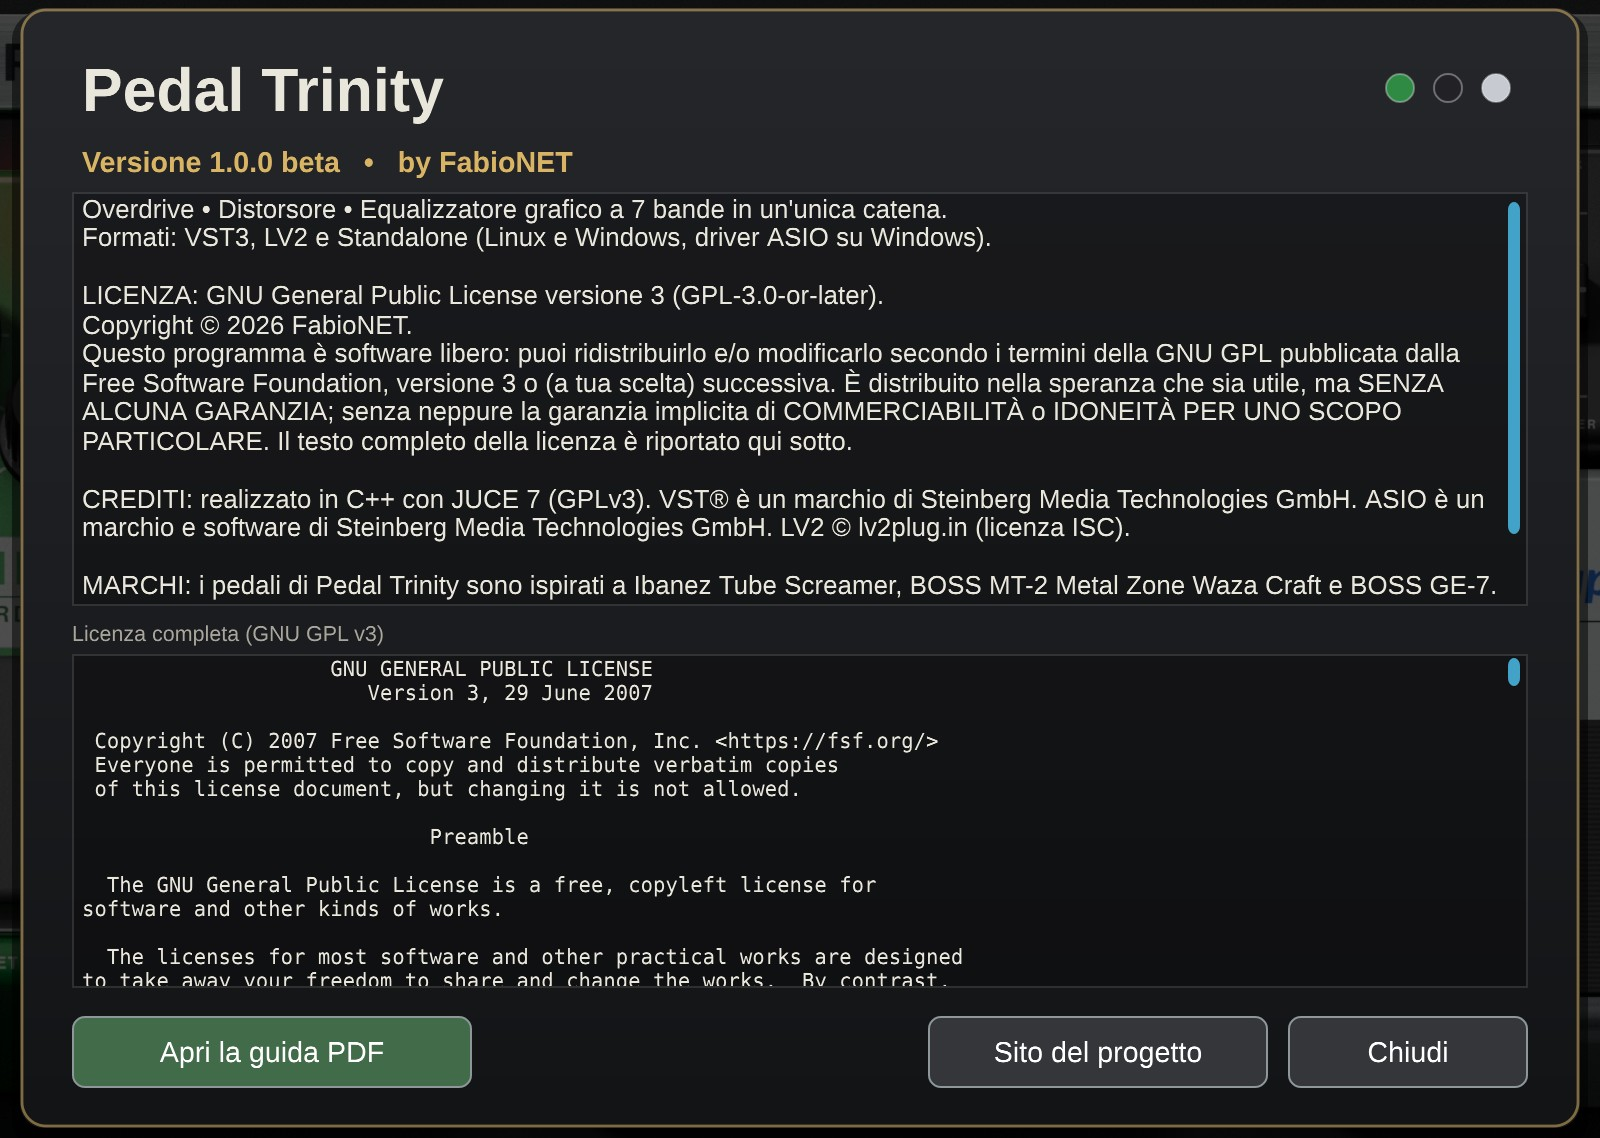
\includegraphics[width=\linewidth]{../images/guide_info.jpg}
\end{minipage}\hfill
\begin{minipage}[t]{0.46\linewidth}\vspace{0pt}
Il tasto \textbf{INFO} sulla targhetta apre la finestra informazioni con:
\begin{itemize}
  \item versione (\textbf{1.0.0 beta}) e autore (\textbf{FabioNET});
  \item riepilogo della licenza e testo completo della \textbf{GNU GPL v3};
  \item crediti e note sui marchi;
  \item il pulsante \textbf{Apri la guida PDF}, che apre questo documento.
\end{itemize}
Chiudi con \textbf{Chiudi}, con il tasto \texttt{Esc} o cliccando fuori dal riquadro.
\end{minipage}

\subsection*{Licenza}
Pedal Trinity è \textbf{software libero}: puoi usarlo, studiarlo, modificarlo e ridistribuirlo secondo i
termini della \textbf{GNU General Public License versione 3} (o successiva) pubblicata dalla Free Software
Foundation. È distribuito nella speranza che sia utile, ma \textbf{senza alcuna garanzia}. Chi ridistribuisce
versioni modificate deve renderne disponibile il codice sorgente con la stessa licenza.
Il codice sorgente è su \url{https://github.com/fabionet/Pedal-Trinity}.

\subsection*{Crediti e marchi}
Realizzato in C++ con JUCE 7 (licenza GPLv3). VST è un marchio di Steinberg Media Technologies GmbH;
ASIO è un marchio e software di Steinberg Media Technologies GmbH. LV2 è uno standard aperto (lv2plug.in).

\emph{Ibanez} e \emph{Tube Screamer} sono marchi di Hoshino Gakki Co.; \emph{BOSS}, \emph{MT-2}, \emph{Metal Zone},
\emph{Waza Craft} e \emph{GE-7} sono marchi di Roland Corporation. Pedal Trinity è un progetto indipendente,
non affiliato né approvato da queste aziende: i nomi servono solo a indicare il suono di riferimento.
Le immagini dei pedali sono render 3D originali.

% ------------------------------------------------------------------
\clearpage
\section{Risoluzione dei problemi}
\begin{tabularx}{\linewidth}{@{}>{\bfseries}p{5.2cm} X@{}}
\toprule
Problema & Soluzione \\ \midrule
Il plugin non compare nella DAW & Ripeti la scansione dei plugin; su Linux verifica che la DAW cerchi in \texttt{/usr/lib/vst3} e \texttt{/usr/lib/lv2}. \\
Nessun suono nello Standalone & In \emph{Options → Audio/MIDI Settings} scegli ingresso e uscita corretti e controlla che \emph{Mute audio input} sia disattivato. \\
Suono in ritardo & Riduci la dimensione del buffer; su Windows usa i driver ASIO. \\
Volume troppo alto/basso & Regola \ctl{LEVEL} del pedale attivo; a 5 il livello è vicino a quello d'ingresso. \\
Crepitii & Aumenta il buffer o riduci il carico della CPU; il suono è elaborato in sovracampionamento 4×. \\ \bottomrule
\end{tabularx}

\vfill
\begin{center}\small\color{steel}
Pedal Trinity 1.0.0 beta \,·\, © 2026 FabioNET \,·\, GNU General Public License v3
\end{center}
\end{document}
